% Exemple de fichier fonctionnnant avec la classe CAp2012.cls
% Base :  
%	Classe pf2010.cls adpatée de pf2003 par Jean CHarlet
%	Classe pf2003.cls adpatée de ic2001 par Jean CHarlet
%
% 	Classe ic2001.cls adpatée de EEGDRI3 par Jean CHarlet
%
% 	Classe EEGDRI3.cls adpatée de ic2000 par Jean CHarlet
%
% 	Classe IC'2000 (ic2000.cls) par Jean Charlet
%
% 	adaptée de la classe IC'99 (afia99.cls) développée par Fabien Torre

%\documentclass{CAp2012}
\documentclass[publibook-draft]{CAp2012}

\newcommand{\verbfichex}{CAp2012.\xspace}
\newcommand{\verbfichclass}{CAp2012.cls\xspace}
\newcommand{\verbfichbst}{CAp2012.bst\xspace}


%\usepackage[pdftex]{pstricks}

\usepackage{verbatim}
\usepackage{subfigure}
\usepackage[french]{babel}
\usepackage[utf8]{inputenc}
\usepackage[T1]{fontenc}
\usepackage{amsmath}
\usepackage{amssymb}

\usepackage{natbib}
\usepackage{algorithm}
\usepackage{algorithmic}
%%% francisation des algorithmes
\renewcommand{\algorithmicrequire} {\textbf{\textsc{Entrées:}}}
\renewcommand{\algorithmicensure}  {\textbf{\textsc{Sorties:}}}
\renewcommand{\algorithmicwhile}   {\textbf{tantque}}
\renewcommand{\algorithmicdo}      {\textbf{faire}}
\renewcommand{\algorithmicendwhile}{\textbf{fin tantque}}
\renewcommand{\algorithmicend}     {\textbf{fin}}
\renewcommand{\algorithmicif}      {\textbf{si}}
\renewcommand{\algorithmicendif}   {\textbf{finsi}}
\renewcommand{\algorithmicelse}    {\textbf{sinon}}
\renewcommand{\algorithmicthen}    {\textbf{alors}}
\renewcommand{\algorithmicfor}     {\textbf{pour}}
\renewcommand{\algorithmicforall}  {\textbf{pour tout}}
\renewcommand{\algorithmicdo}      {\textbf{faire}}
\renewcommand{\algorithmicendfor}  {\textbf{fin pour}}
\renewcommand{\algorithmicloop}    {\textbf{boucler}}
\renewcommand{\algorithmicendloop} {\textbf{fin boucle}}
\renewcommand{\algorithmicrepeat}  {\textbf{répéter}}
\renewcommand{\algorithmicuntil}   {\textbf{jusqu'à}}

\floatname{algorithm}{Algorithme}


%\newtheorem{algorithm}{Algorithme}
\newtheorem{definition}{Définition}

%%%%%%%%%%%%%%%%%%%%%%%%%%%%%%%%%%%%%%%%%%%%%%%%%%%%%%%%%%%%%%%%%%%%%%%
% Titre court si le titre fait plus de 40 caractères
%%%%%%%%%%%%%%%%%%%%%%%%%%%%%%%%%%%%%%%%%%%%%%%%%%%%%%%%%%%%%%%%%%%%%%%

\shorttitle{Batch Inverse Reinforcement Learning}

\shortouvrage{CAp 2012}

% Titre, auteur, pas de date

\title{Batch Imitation via Inverse Reinforcement Learning Without Solving the Direct Problem}

\author{\fontsize{12}{12}\selectfont{Edouard Klein\inst{1}\inst{2}, Matthieu Geist\inst{1}, Olivier Pietquin\inst{1}\inst{3}}}

\institute{
Sup\'elec,\\
IMS Research group, France\\
\texttt{prenom.nom@supelec.fr}
\and
Equipe ABC,\\
LORIA-CNRS, France
\and
UMI 2958\\
GeorgiaTech-CNRS, France
}


\begin{document}
\maketitle


\begin{abstract}
  Cette publication s'occupe du problème de l'apprentissage par imitation par le biais de l'apprentissage par renforcement inverse ({\it Inverse Reinforcement Learning, IRL}). Dans ce contexte, un expert accomplit une tâche qu'un agent doit essayer de reproduire. L'IRL part du postulat que l'expert optimise avec succès une fonction d'utilité et cherche à deviner cette fonction (appelée récompense) avec pour entrée une trace du comportement de l'expert. Les algorithmes d'IRL existant nécessitent une ou plusieurs des conditions suivantes pour fonctionner : trajectoires complètes de la part de l'expert, un modèle génératif pour les estimations de type Monte-Carlo, la connaissance des probabilités de transition et la capacité de résoudre le problème direct (celui du {\it Reinforcement Learning, RL}) de manière répétée. Notre contribution est la présentation d'un nouvel algorithme d'IRL levant toutes ces contraintes. En utilisant méthode supervisée dans laquelle nous introduisons la structure du processus décisionnel de Markov ({\it Markov Decision Process, MDP}) sous-jacent, nous créons un algorithme basé sur une descente de sous gradient et possèdant une faible complexité tant en échantillons que calculatoire.
  \motscles{Apprentissage par renforcement, Apprentissage par renforcement inverse, Processus Decisionnel de Markov}
\end{abstract}
\section{Introduction}
\begin{itemize}
\item Introduction informelle sur les processus de décision séquentiels
\item Intérêt de l'Apprenticeship learning
\item Intérêt de l'IRL pour faire de l'apprenticeship learning
\item Rapide point sur les limitations des algos d'IRL actuels
\begin{itemize}
\item \cite{ng2000algorithms} : Probabilités de transitions devant être connues
\item \cite{abbeel2004apprenticeship} et toutes les approches résumées dans \cite{neu2009training}: Résolution du problème direct à chaque itération
\end{itemize}
\end{itemize}
\section{Background}
\label{back.sec}
\begin{itemize}
\item Introduction rapide, pour les notations, des MDPs, du RL et de l'IRL
\end{itemize}
\section{Loss-augmented Feature Expectation Matching}
\subsection{Principe}
Notre algorithme cherche à minimiser la fonction de risque suivante :
\begin{equation}
  R_N(q) = {1\over N} \sum_{i=1}^N\left(\max_{a}(q(s_i,a) + l(s_i,a)) - q(s_i,a_i) \right)
\end{equation}
Dans le travail de \citep{ratliff2007imitation}, cette fonction de risque est introduite pour décrire un classifieur utilisant la fonction de score $q$ et qui à un élément $s$ associe la label $a = \arg\max\limits_a q(s,a)$. Cela est très similaire à l'équation
  \begin{equation}
  \label{greedy.eqn}
  \pi^*(s) = \arg\max_{a} Q^*(s,a)
  \end{equation}
  qui décrit le mécanisme glouton liant fonction de valeur optimale et politique optimale. La politique de l'expert étant une politique optimale, elle doit respecter cette équation. Minimiser notre fonction de risque revient donc à chercher une fonction $q$ compatible avec la fonction de valeur optimale de l'expert. En effet, considérons que la fonction de perte $l$ est uniformément nulle et regardons ce qui se passe lorsque la fonction de risque $R_N(q)$ est minimisée. On introduit $a^* = \arg\max\limits_a(q(s_i,a))$. Si la fonction de risque $R_N(q)$ est positive, alors il arrive pour certains $i$ que $q(s_i,a^*) > q(s_i,a_i)$. Cela signifie que la fonction $q$ ne permet pas de justifier le choix de l'expert. A l'opposé, si l'on parvient à anuller $R_N(q)$, on a $\forall i, q(s_i,a^*) = q(s_i,a_i)$, et donc $a_i \in \arg\max\limits_a q(s_i,a)$, ce qui justifie le choix de l'expert.\\

   La fonction de perte $l$ permet d'introduire de la connaissance à priori en laissant l'opérateur influer sur la forme de la fonction $q$ recherchée.\\

   Nous allons profiter de la structure présente dans $Q$ pour introduire la notion de \emph{feature expectation} dans le problème. On rappelle qu'en IRL il est classique d'écrire $Q(s,a) = \theta^T \mu(s,a)$. Nous nous basons donc sur la \emph{feature expectation} de l'expert, $\mu_E$ et un vecteur de paramètres $\theta$ contrôlant la fonction de récompense que l'on recherche pour réécrire la fonction de risque que nous allons minimiser :
  \begin{equation}
   R_N(\theta) = {1\over N} \sum_{i=1}^N\left(\max_{a}(\theta ^T \mu_E(s_i,a) + l(s_i,a)) - \theta ^T \mu_E(s_i,a_i) \right)
   \end{equation}
   Il faut noter ici l'utilisation non pas de $\mu_E : S\rightarrow \mathbb{R}^p$ mais de $\mu_E : S\times A \rightarrow \mathbb{R}^k$. Cette dernière partage avec la première la même relation que $Q$ partage avec $V$, c'est à dire que l'on dispose d'un degré de liberté en plus correspondant à la prochaine action, qui peut différer de celle choisie par l'expert.

   
   De la même manière que précedemment, on note $a^* = \arg\max\limits_{a} = \theta_t ^T \mu_E(s_i,a) + l(s_i,a)$, l'expression de la fonction de risque devient alors :
   \begin{eqnarray}
   R_N(\theta) &=& {1\over N} \sum_{i=1}^N\left(\theta ^T \mu_E(s_i,a^*) + l(s_i,a^*) - \theta ^T \mu_E(s_i,a_i) \right)\\
   &=& {1\over N} \sum_{i=1}^N\left(\theta^T\left(\mu_E(s_i,a^*) - \mu_E(s_i,a_i)\right) + l(s_i,a^*)  \right).
   \end{eqnarray}

   La présence d'un $\max$ dans cette expression (caché dans le $a^*$) nous oblige à utiliser le sous gradient dont la règle est que le sous gradient du $\max$ est le gradient de l'$\arg\max$.

   Le sous gradient de cette expression est donc : 
   \begin{equation}
   \nabla L_N(\theta) =  {1\over N}\sum_{i=1}^N\left(\mu_E(s_i,a^*) - \mu_E(s_i,a_i)\right).
   \end{equation}

   Une descente de gradient sur le risque donne la règle d'update suivante :
   \begin{equation}
   \theta_{t+1} = \theta_t -\alpha_t{1\over N}\sum_{i=1}^N\left(\mu_E(s_i,a^*) - \mu_E(s_i,a_i)\right),
   \end{equation}

   avec $\alpha_t$ un pas d'apprentissage. L'algorithme complet est détaillé algorithme \ref{LAFEM.alg}.

\begin{algorithm}
\caption{LAFEM ({\it Loss-Augmented Feature Expectation Matching})}
\label{LAFEM.alg}
\begin{algorithmic}
  \REQUIRE une fonction de perte $l : S\times A \rightarrow \mathbb R$
  \REQUIRE la \emph{feature expectation} de l'expert $\mu_E : S\times A \rightarrow \mathbb R ^p$
  \REQUIRE un pas d'apprentissage $\alpha : \mathbb N \rightarrow \mathbb R$
  \REQUIRE des données provenant de l'expert $\{(s_i,a_i)\}_{i=1..N}$
  \REQUIRE un vecteur de paramètres initial $\theta_0$
  \REQUIRE un nombre maximum d'itérations $T\in \mathbb N$
  \REQUIRE une description de l'espace d'action $A$

     
  \FOR {T iterations}
  \STATE $\Delta\theta \leftarrow [0...0]^T$
    \FORALL{ $(s_i,a_i)$}
    \STATE $a^* \leftarrow \arg\max\limits_{a} = \theta_t ^T \mu_E(s_i,a) + l(s_i,a)$
    \STATE $\Delta\theta \leftarrow \Delta\theta + \mu_E(s_i,a^*) - \mu_E(s_i,a_i)$
    \ENDFOR
    \STATE $\theta_{t+1} = \theta_t -\alpha_t{1\over N}\Delta\theta$
    \ENDFOR
    \RETURN $\theta_T$
\end{algorithmic}
\end{algorithm}
\section{Experimental results}
\subsection{GridWorld}
\begin{itemize}
\item Description du setting (GridWorld, expert, nombre de trajectoires, etc.)
\item Description des réglages de LAFEM (fonction $l$ notamment, calcul exact de $\mu_E$)
\item Présentation des résultats (pas grand chose à dire)
\end{itemize}
\begin{figure}
\begin{minipage}[t]{.4\linewidth}
    \begin{center}
       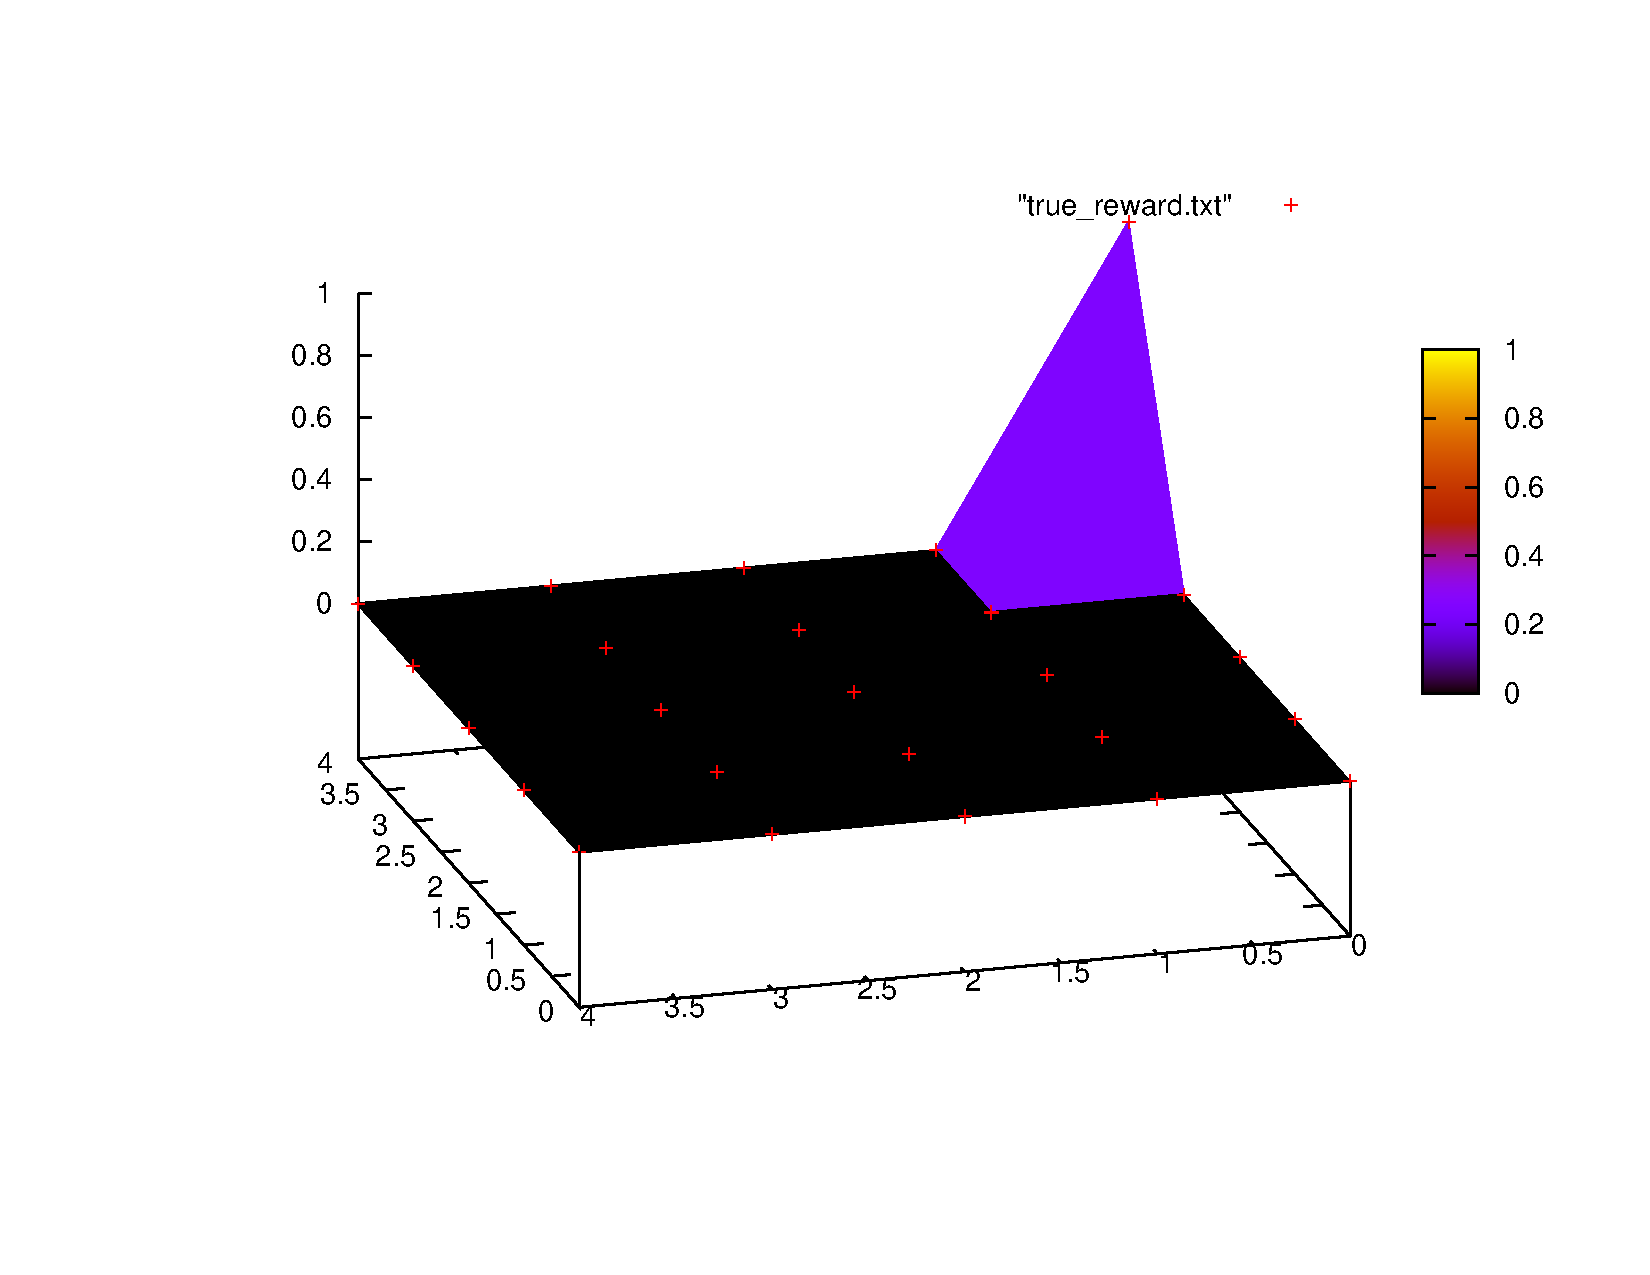
\includegraphics[width=\textwidth]{../GridWorld/true_reward.pdf}
       \caption{Expert's reward}
       \label{nbabo}
    \end{center}
\end{minipage}
\hfill
\begin{minipage}[t]{.4\linewidth}
    \begin{center}
       \includegraphics[width=\textwidth]{../GridWorld/retrieved_reward.pdf}
       \caption{Reward found by LAFEM}
       \label{croissnbabo}
    \end{center}
\end{minipage}\\
\begin{minipage}[t]{.4\linewidth}
    \begin{center}
       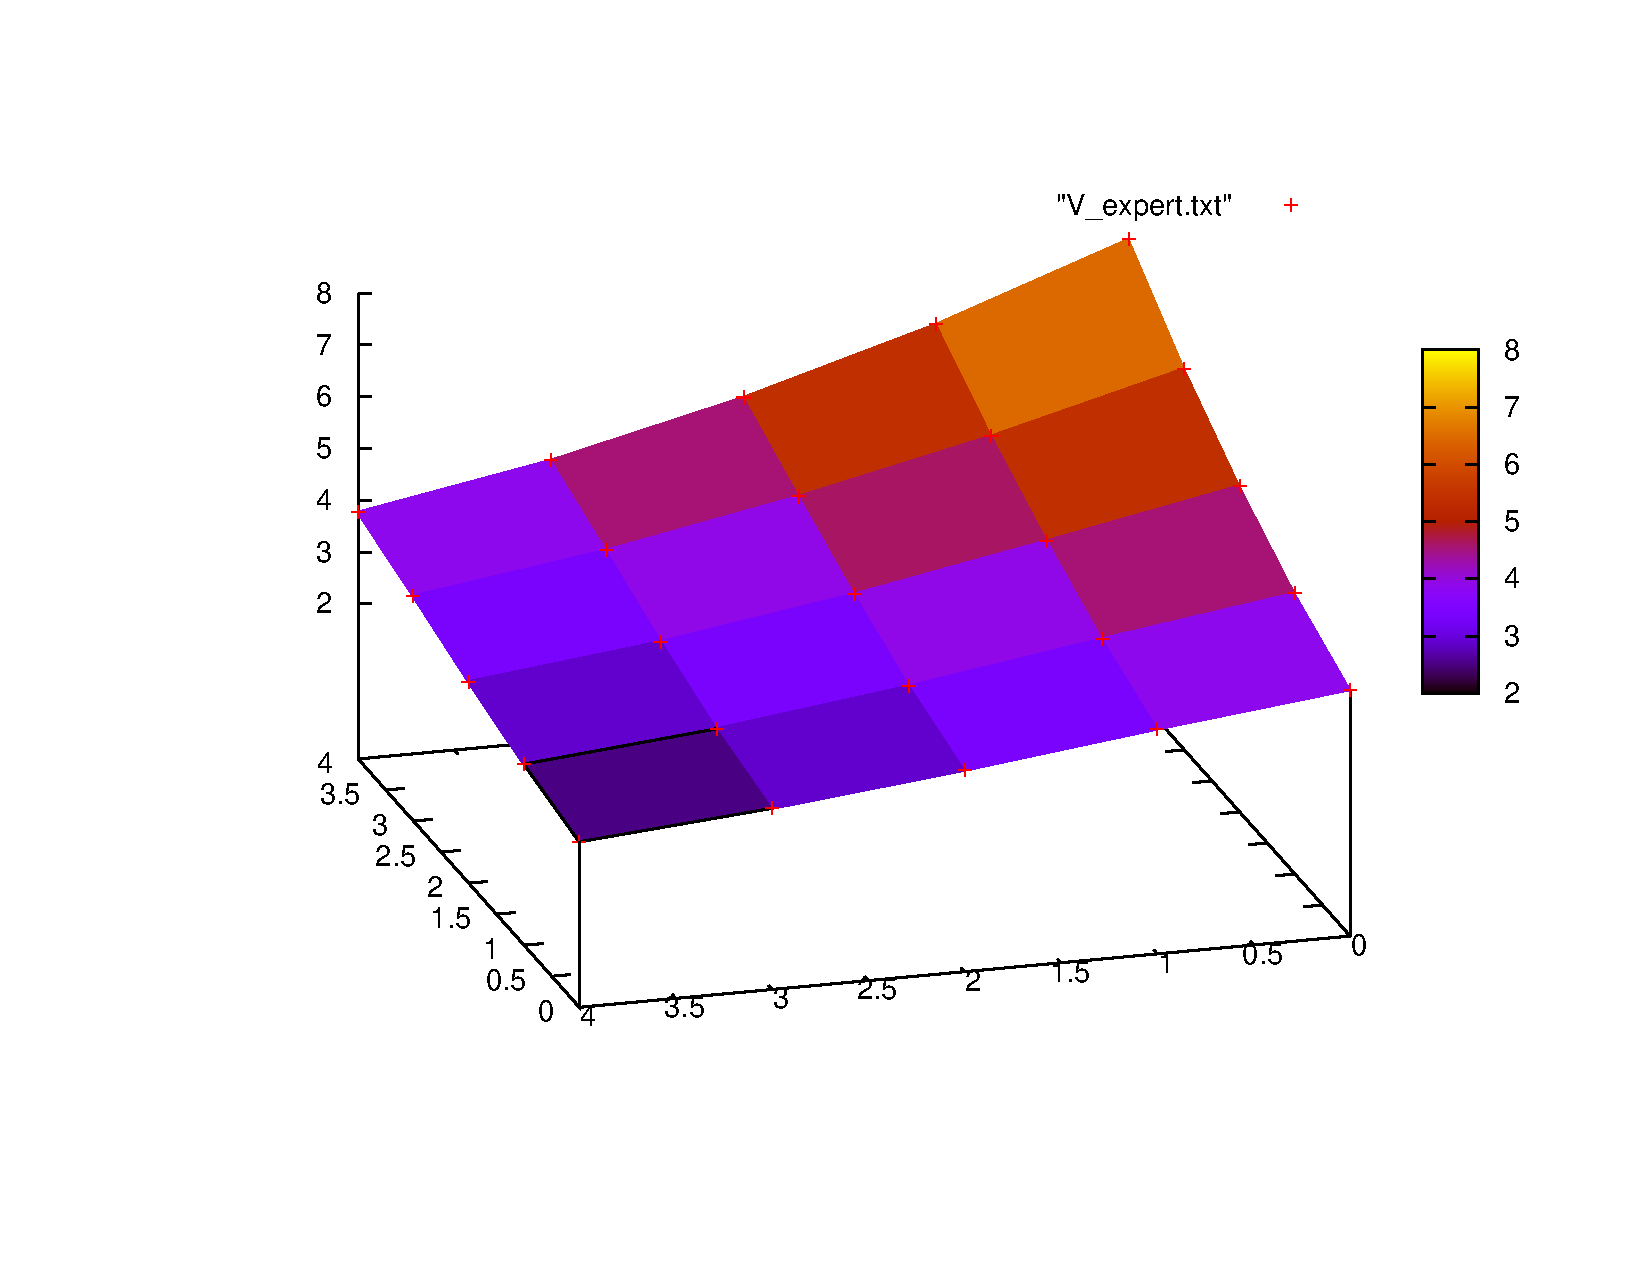
\includegraphics[width=\textwidth]{../GridWorld/V_expert.pdf}
       \caption{Expert's reward}
       \label{nbabo}
    \end{center}
\end{minipage}
\hfill
\begin{minipage}[t]{.4\linewidth}
    \begin{center}
       \includegraphics[width=\textwidth]{../GridWorld/V_agent.pdf}
       \caption{Agent's value function}
       \label{croissnbabo}
    \end{center}
\end{minipage}\\

\end{figure}

\subsection{Inverted Pendulum}
\begin{itemize}
\item Présentation du setting (Le pendule, l'expert)
\item Réglages de LAFEM (Préciser l'utilisation de LSTD$\mu$)
\item Présentation des résultats
\item Discussion sur la variabilité de la récompense
\item Présentation des performances statistiques (expérience pas encore effectuée)/ Etude de la complexité en échantillons 
\item Pas de comparaison avec le travail de \cite{abbeel2004apprenticeship} car celui-ci ne marche tout simplement pas avec les informations dont on dispose
\end{itemize}
\section{Related Work}
\begin{itemize}
\item Résumé plus détaillé que précédemment des approches IRL actuelles
\item Laïus sur Ratliff et son approche locale (imitation pure) et globale (plain de contraintes)
\end{itemize}
\section{Conclusion and future work}
\begin{itemize}
\item On enlève les contraintes du domaine d'un seul coup, 
\item Il ne reste que la sélection ou détection de features, mais ce n'est pas hors de portée
\item Dans la même veine, il reste la résolution du problème direct une fois la récompense obtenue, il faut peut-être creuser du côté du reward shaping
\item Faible complexité computationnelle
\item Faible complexité en échantillons
\item Il reste des tests à faire sur le Highway driving (Pour ICML ?) et sur des expériences dans la vraie vie (bras robot ?) pour comparer à l'existant
\end{itemize}
%
% Bibliographie
%
\bibliography{../../Biblio/Biblio}

\end{document}

